\chapter{Mở đầu}
\section{Đặt vấn đề}
  Ngày nay, các công cụ tìm kiếm như Google hay Bing hoạt động bằng cách tìm kiếm và truy xuất thông tin từ hàng tỷ trang web trên Internet và cung cấp kết quả phù hợp cho người dùng. Để làm được điều này, chúng sử dụng các thuật toán tìm kiếm, một tập hợp các quy tắc và quy trình xử lí để xác định, sắp xếp các kết quả tìm kiếm. Trong đó phải kể đến thuật toán tìm kiếm của công cụ tìm kiếm Internet Google - ra đời 1997. Thuật toán đó đã đóng vai trò then chốt đưa Google trở thành công cụ dẫn đầu trong cuộc chiến tìm kiếm. Thuật toán đó được đặt tên là \textbf{PageRank}, được giới thiệu qua bài báo cáo năm 1998 của Larry Page và Sergey Brin tại Đại học Stanford. 
  
  Hiện nay, các địa chỉ trang web được tổ chức theo cấu trúc \emph{Web Search} và tìm kiếm dựa trên các \emph{search phrase}. Khi đó các công cụ tìm kiếm hoạt động bằng cách thu thập thông tin của các trang web, liệt kê các từ khóa và đưa vào trong một cấu trúc lưu trữ gọi là \emph{inverted index} (chỉ mục đảo ngược)\cite{Leskovec_Rajaraman_Ullman_2022}. \emph{Inverted index} sẽ tạo một sơ đồ liên kết giữa từ khóa và các tài liệu chứa từ khóa đó. Thông qua đó, ta có một thuật toán tìm kiếm đơn giản bằng cách thực hiện phép giao giữa các chỉ mục. Nhưng điều này tạo ra một lỗ hổng mà bị kẻ xấu lợi dụng để đánh lừa các công cụ tìm kiếm. Phương pháp đánh lừa đó gọi là \emph{term spam}, một cách sử dụng các từ khóa phổ biến nhằm điều hướng các tìm kiếm dẫn đến trang web của họ. Các công cụ tìm kiếm lúc này trở nên vô dụng và đưa ra kết quả sai lệch. Khi đó Larry Page và Sergey Brin đã đưa ra 2 cải tiến:
  \begin{enumerate}    
    \item \textbf{Thuật toán PageRank}: qua mô hình mô phỏng quá trình người dùng duyệt web, từ 1 trang web, di chuyển ngẫu nhiên theo các \emph{outgoing links} đến các trang khác và lặp lại nhiều lần. Các trang có số lượng truy cập lớn sẽ được đánh giá là \textbf{quan trọng} hơn và sẽ được ưu tiên hiển thị trong kết quả tìm kiếm.\cite{Leskovec_Rajaraman_Ullman_2022}
    \item Một trang được đánh giá không chỉ bởi các từ khóa trên trang đó mà còn qua các từ khóa sử dụng trong các trang có liên kết gần với trang đó.\cite{Leskovec_Rajaraman_Ullman_2022}
  \end{enumerate}
  Nhờ cải tiến đó, vấn đề \emph{term spam} đã được giải quyết. Việc đánh giá thông qua cả nội dung và các trang liên kết giúp việc bị đánh lừa khó diễn ra hơn. Và các trang web giả mạo, dù có nhiều liên kết giả, vẫn sẽ bị thuật toán đánh giá thấp.
  
  Từ đó đến nay, thuật toán PageRank đã được chứng minh bằng thực nghiệm là có tác dụng, và vì vậy chúng ta sẽ nghiên cứu chi tiết cách tính toán và hình thành nó.
%----------------------------------------------------------------------- ||
%%%%%%%%%%%%%%%%%%%%%%%%%%%%%%%%%%%%%%%%%%%%%%%%%%%%%%%%%%%%%%%%%%%%%%%% ||
%----------------------------------------------------------------------- ||
\section{Thuật toán PageRank}
  Thuật toán PageRank là một thuật toán mà sẽ ước tính và gán cho mỗi trang web một số thực dựa trên mức độ quan trọng của nó. Con số đó được gọi là PageRank của một trang web. Một trang web có PageRank càng cao thì nó càng \textbf{quan trọng}.
  \begin{align}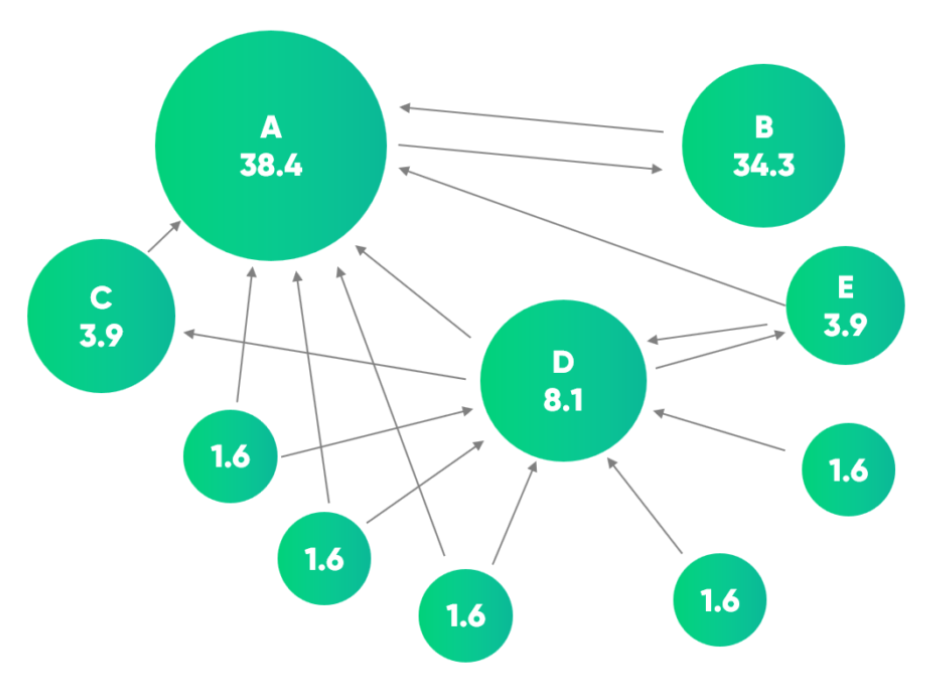
\includegraphics[width=0.5\textwidth]{figure/pagerank-example.png}\end{align}
  Thuật toán không dừng lại chỉ ở việc đánh giá một trang web bằng số lượng \emph{incoming links}, mà còn dựa trên PageRank của các trang web dẫn đến nó.
  
  Thuật toán PageRank dựa trên phương pháp gọi là \emph{Random Surfer Model} - mô hình mô phỏng khả năng người dùng truy cập ngẫu nhiên đến các \emph{outgoing links} từ một trang web cụ thể. Ý tưởng cho phương pháp như sau:
  \begin{itemize}
      \item Bắt đầu ở một trang ngẫu nhiên, từ đó, đi qua liên kết bất kì đến một trang khác (tỉ lệ truy cập đến mỗi \emph{outgoing link} là như nhau). Thực hiện lặp lại, và thực hiện đếm số lần mà mô hình truy cập đến 1 trang cụ thể. Và dễ thấy một trang có nhiều \emph{incoming links} hơn sẽ có lượng truy cập đếm được lớn. Ngoài ra, các trang mà được liên kết từ các trang có truy cập lớn cũng sẽ mang lượng truy cập lớn. Vì vậy liên kết từ một trang có nhiều truy cập sẽ có giá trị hơn liên kết từ một trang có lượng truy cập thấp hơn\cite{YouTube_2020}.
      \item Sau số lần lặp nhất định, dựa vào lượng truy cập đã có của từng trang, ta có được giá trị tương đối về độ quan trọng của trang đó thông qua tỉ lệ phần trăm thời gian mà mô hình truy cập ngẫu nhiên truy cập đến đó.
  \end{itemize}
  
  Không có một thuật toán cố định nào để đánh giá một trang web. Có nhiều biến thể khác nhau của thuật toán, được cải tiến dựa trên thực tế sử dụng và khắc phục các điểm yếu. Ví dụ như Google với PageRank và Baidu với RankDek, cả hai đều dựa trên ý tưởng tương tự nhau. Trong báo cáo, chúng ta sẽ tìm hiểu chi tiết về thuật toán PageRank do hai nhà sáng lập của Google đưa ra.

%170523
%200523

  
